\documentclass[11pt]{article}
\usepackage[margin=2.5cm]{geometry}
\usepackage{array,booktabs,enumitem,graphicx,url,amsmath}
\renewcommand{\arraystretch}{1.12}
\newcolumntype{L}[1]{>{\raggedright\arraybackslash}p{#1}}
\graphicspath{{../outputs/eda_charts/}}

\title{SmogShield Lahore: Deliverable 1\\Problem Definition and Data Foundations}
\author{Muhammad Haider Mughal (3006) \and Muhammad Ayub Butt (3076) \and Abdul Rehman (3059)}
\date{}

\begin{document}
\maketitle
% Phase 1: Problem Definition (included by report_main_final.tex).
% Needs in the main file's preamble: \usepackage{array,booktabs,enumitem}
% and this line:  \newcolumntype{L}[1]{>{\raggedright\arraybackslash}p{#1}}
% Citations resolve against the thebibliography block in report_main_final.tex.

\section{Phase 1: Problem Definition}

\subsection{Problem Statement}

Lahore experiences recurring episodes of severe air pollution, most visibly during the winter ``smog season'' that roughly spans October to February~\cite{majeed2024lahore}. The pollutant most often used to describe these episodes is fine particulate matter (PM$_{2.5}$), particles smaller than 2.5~$\mu$m that can be inhaled deeply~\cite{who2024ambient,epa_pm_basics}.

Our own data shows how persistent the problem is. The US Diplomatic Post monitor in Lahore recorded at least 18 valid hourly readings on 1{,}506 days between May 2019 and March 2025. Converting each day's mean PM$_{2.5}$ to the US EPA Air Quality Index (AQI, 2012 breakpoints)~\cite{epa_aqi_tad}, only 9 of those days (0.6\%) fell in the ``Good'' category, while 1{,}102 days (73.2\%) were ``Unhealthy'' or worse. These figures come from a single monitor and from days with enough valid readings, so they describe the data we have rather than the whole city.

\paragraph{The pain point.} A resident deciding whether to cycle to work, hold a school sports session, or work outdoors tomorrow needs three things: a forecast, an idea of how reliable it is, and a reason for it. Air-quality information is commonly presented as a current reading, which leaves three gaps:
\begin{itemize}
  \item \textbf{Timing:} a current value does not say what tomorrow will look like.
  \item \textbf{Trust:} a single number gives no sense of how uncertain it is.
  \item \textbf{Understanding:} people are rarely told which conditions (for example calm air, cold temperatures, high humidity) are driving the pollution.
\end{itemize}

\paragraph{Our solution.} SmogShield Lahore is a web application that forecasts the next day's PM$_{2.5}$ level and AQI category for Lahore from historical air-quality and weather data (with calendar-based proxies where traffic data is unavailable). Each forecast comes with a prediction interval, the main factors the model relied on, and cautious, non-medical guidance. The project also studies recurring seasonal pollution patterns and tests whether adding weather and calendar information improves forecast accuracy.

\subsection{Target Audience}

\begin{table}[h]
\centering
\small
\begin{tabular}{L{3.6cm}L{4.6cm}L{5.6cm}}
\toprule
\textbf{User group} & \textbf{Decision they face} & \textbf{What SmogShield provides} \\
\midrule
Commuters, cyclists and runners & Whether to travel or exercise outdoors tomorrow & Next-day AQI category with an uncertainty range \\
Parents and schools & Whether to hold outdoor activities & Category-based, cautious guidance \\
Outdoor workers & Planning the working day & Forecast and typical cleaner hours from historical patterns \\
Residents who may be sensitive to air pollution, and their carers & Deciding how cautious to be & The forecast category and the factors behind it (not medical advice) \\
Students and researchers & Assessing a transparent baseline & Documented data, models and limitations \\
\bottomrule
\end{tabular}
\caption{Target users and how the application supports their decisions.}
\end{table}

The primary audience is the general public in Lahore. SmogShield is not a medical tool and does not replace official public-health advisories.

\subsection{AI Justification}

A rule-based system would encode expert thresholds such as ``if wind speed is below X and humidity is above Y, predict poor air quality.'' Machine-learning models have already been used to forecast Lahore's AQI from historical series~\cite{waqas2024lahore}; SmogShield extends this line by forecasting next-day PM$_{2.5}$ with weather and calendar inputs and by attaching uncertainty and explanations to each forecast. We argue that machine learning is better suited to this problem for the following reasons.

\begin{enumerate}
  \item \textbf{Many interacting factors.} Tomorrow's PM$_{2.5}$ depends on today's level and on wind speed and direction, humidity, dew point, temperature, pressure, rainfall and the time of year. The effect of one factor depends on the others (for example, calm air matters most when it is also cold and humid). Writing and justifying thresholds for every combination by hand does not scale, whereas learning algorithms such as tree ensembles fit these interactions directly from data.
  \item \textbf{Relationships change with the season.} The same wind speed does not mean the same thing in a monsoon July and in a December smog episode. Rules would need separate hand-tuned sets for each regime. A model trained on several years of data can learn these differences.
  \item \textbf{Uncertainty has to be estimated.} A fixed rule gives a single answer. Learned models allow prediction intervals to be estimated from historical forecast errors (for example with quantile regression), which supports the trust gap described above.
  \item \textbf{The data is suitable.} We have an observed daily PM$_{2.5}$ series with 1{,}506 usable days, together with more than 2{,}600 days of daily weather. This is a tabular supervised learning problem with enough rows for tree-based models and regularised linear models, and possibly a small recurrent network for comparison.
  \item \textbf{Maintainability.} When new data arrives, a model can be retrained and re-evaluated. A rule set must be re-tuned manually.
  \item \textbf{Complement to physical models.} Atmospheric models exist, but a modeled air-quality dataset we examined during Phase 2 read about half as high as the monitor on overlapping days and under-read smog peaks. A statistical model trained on local observations is a practical complement.
\end{enumerate}

\paragraph{An honest counterpoint.} Daily pollution is strongly persistent, so a simple baseline that predicts ``tomorrow equals today'' is hard to beat. For this reason we compare every learned model against that persistence baseline and against simple linear models. We claim a benefit from machine learning only where the evaluation shows one.

\begin{table}[h]
\centering
\small
\begin{tabular}{L{4.0cm}L{4.9cm}L{4.9cm}}
\toprule
\textbf{Aspect} & \textbf{Rule-based} & \textbf{Machine learning} \\
\midrule
Factor interactions & Hand-written, limited & Learned from data \\
Seasonal differences & Separate rule sets & Learned, can use season as input \\
Uncertainty & Not provided & Estimated from past errors \\
Updating & Manual re-tuning & Retrain on new data \\
Evidence of accuracy & Hard to measure fairly & Compared with baselines on held-out data \\
\bottomrule
\end{tabular}
\caption{Why a learned model is preferred over fixed rules for this problem.}
\end{table}

\subsection{Research Questions and Scope}

\begin{enumerate}
  \item[\textbf{RQ1}] Can machine learning models forecast next-day PM$_{2.5}$ and AQI category better than a persistence baseline?
  \item[\textbf{RQ2}] Does adding weather, and then calendar information, improve accuracy compared with air-quality history alone (ablation study)?
  \item[\textbf{RQ3}] Where do the models fail? We examine errors by season and on extreme-pollution days.
\end{enumerate}

\paragraph{Scope and limitations.} The forecast is for the next day at daily resolution, for Lahore, based mainly on one reference monitor. Traffic is represented by calendar proxies because no open, time-aligned Lahore traffic dataset was found. The data has gaps, and the evaluation uses a time-based split so that no future information leaks into training. The application gives cautious guidance and is not medical advice.

% References are listed in the thebibliography block of report_main_final.tex.

% Phase 2: Data Foundations (included by report_main_final.tex).
% Needs in the main file's preamble:
%   \usepackage{array,booktabs,enumitem,graphicx,url,amsmath}
%   \newcolumntype{L}[1]{>{\raggedright\arraybackslash}p{#1}}
%   \graphicspath{{processed/eda_charts/}}

\section{Phase 2: Data Foundations}

Phase 2 turns the problem definition into a documented, reproducible dataset. This section records where every file came from, what was cleaned and why, how variables are encoded for modelling, and what the exploratory analysis shows about Lahore's PM$_{2.5}$.

\subsection{Data Collection}

\paragraph{Sources.}
Table~\ref{tab:sources} lists the five data products. We combine a measured target series with meteorological features and two modelled products that serve as validation; the modelled products are never treated as ground truth.

\begin{table}[htbp]
\centering
\footnotesize
\begin{tabular}{@{}L{2.7cm}L{4.4cm}L{2.2cm}L{1.3cm}L{1.6cm}@{}}
\toprule
\textbf{Dataset} & \textbf{Source and access} & \textbf{Coverage} & \textbf{Rows} & \textbf{Licence} \\
\midrule
OpenAQ hourly PM$_{2.5}$ & OpenAQ v3 API, sensor 25135 (US Diplomatic Post, Lahore) & 22 May 2019 -- 4 Mar 2025 & 46{,}465 hourly & Provider-specific \\
ERA5 daily weather & Open-Meteo Historical Weather API, model \texttt{era5} & 1 Jun 2019 -- 7 Oct 2026 & 2{,}686 daily & CC BY 4.0 \\
Station AQI + weather & GitHub \path{taimoorbarlas15/Lahore_Air_Quality} & 1 Jun 2019 -- 30 Nov 2023 & 1{,}644 daily & Not stated \\
CAMS hourly (modelled) & Kaggle \path{aadbutt/dataset}; regenerable from the Open-Meteo Air-Quality API & 1 Jan 2023 -- 1 May 2025 & 20{,}448 hourly & Unknown / CC BY 4.0 \\
CAMS daily (modelled) & Zenodo DOI 10.5281/zenodo.18673725 & 1 Aug 2022 -- 18 Feb 2026 & 1{,}298 daily & CC0-1.0 \\
\bottomrule
\end{tabular}
\caption{Data sources used in Phase 2.}
\label{tab:sources}
\end{table}

\paragraph{How the data was obtained.}
The API-based sources are downloaded by \path{data_scripts/01_download_data.py}, which uses only the Python standard library. OpenAQ data is requested in 90-day chunks with pagination and retries; the key is read from the \texttt{OPENAQ\_API\_KEY} environment variable and is never written into the code or the repository. The Open-Meteo requests are chunked where a single response would be too large. The Zenodo archive and the GitHub station file are downloaded directly.

\paragraph{Reproducibility and storage.}
Every delivered raw file is fingerprinted with SHA-256 in \path{reports/data_collection_log.md}. Re-running the collection script reproduced the station file and all three Zenodo files byte-for-byte; the ERA5 and CAMS sources are live and may be revised slightly, so they are equivalent rather than necessarily identical. Raw files are kept on the shared Google Drive folder and are excluded from GitHub; only scripts, documentation and derived outputs are version-controlled.

\paragraph{Why several sources.}
OpenAQ provides the measured target. ERA5 supplies the weather features that Phase~1 identified as physically relevant. The GitHub station file offers an independent cross-check of AQI and weather over 2019--2023: daily AQI computed from the OpenAQ series agrees with it over 1{,}153 shared days, with a correlation of 0.99 and a mean absolute difference of 9.3 AQI points. The two CAMS products quantify how far a modelled air-quality product is from the monitor, which is useful context for the ``complement to physical models'' argument in Phase~1.

\subsection{Data Cleaning Implementation}

\paragraph{Scope.}
Cleaning covers missing values, duplicate records, impossible or extreme values, and the standardisation of dates and units. Combining columns is feature engineering and is described in Section~\ref{sec:features}. Missing values are left as missing rather than imputed: fabricating a smog peak would bias both the forecast and the evaluation.

\paragraph{Code.}
The steps below are implemented in \path{data_scripts/}: \path{02_clean_pm25_simple.py} and \path{03_pm25_aqi_and_eda.py} (OpenAQ series, daily aggregation, AQI and the EDA charts), \path{04_clean_station_simple.py} (station file), three scripts numbered 05--07 (ERA5 weather and the two CAMS files; the CAMS hourly timestamps are UTC and are converted to Pakistan time), \path{08_build_calendar.py} (calendar table) and \path{09_build_features.py} (feature table). Each script prints before-and-after counts.

\subsubsection{OpenAQ hourly PM$_{2.5}$}

The raw file contains 46{,}465 hourly records. There are no duplicate timestamps, no negative values and no values above 1{,}000~$\mu$g/m$^3$; the maximum is 974~$\mu$g/m$^3$, which is a plausible extreme smog reading rather than a data error. A total of 8{,}997 values (19.4\%) are empty, a further 4{,}238 hours between the first and last timestamp have no record at all, and 9{,}596 records carry OpenAQ quality flags, of which 1{,}018 still contain a value.

We aggregate the hourly series to local calendar days (Pakistan Standard Time, UTC+5). A day is \emph{usable} when it has at least 18 valid hourly readings; this leaves 1{,}506 usable days out of the 2{,}113 calendar days spanned by the file. The daily value is the mean of the valid hours, and the daily AQI is computed from that mean with the US EPA 2012 breakpoints. Flagged values are retained for now; a sensitivity test that excludes them is planned for the modelling phase.

\subsubsection{Station file}

The station file has 1{,}644 daily rows and 17 columns. Three problems were fixed. First, dates are stored as \texttt{dd-mm-yy}; they were parsed with an explicit \texttt{\%d-\%m-\%y} format, because allowing pandas to infer the format misparsed 594 of the 1{,}644 days. Second, temperatures are in Fahrenheit, wind speeds in miles per hour and pressure in inches of mercury; these were converted to degrees Celsius, kilometres per hour and hectopascals. Third, zeros in the minimum-temperature, minimum-dew-point, minimum-humidity and minimum-pressure columns are physically impossible in Lahore (53, 53, 61 and 127 cells respectively), and spikes in the maximum columns (for example a maximum temperature of 196~$^\circ$F) fall outside physical limits; in total 323 impossible values were set to missing. Gaps of at most three days in the daily average weather columns were filled from the previous day. The AQI itself is never filled: only 2 of the 221 missing AQI values fall on days with a usable PM$_{2.5}$ value in the OpenAQ series, so they stay missing.

\subsubsection{Weather and modelled datasets}

The ERA5 file contains three metadata lines followed by 2{,}686 daily rows; it has no duplicate dates and no missing cells after the empty trailing row for 8 October 2026 is dropped. The CAMS hourly file has 20{,}448 rows with no duplicates, missing cells or negative values. The CAMS daily file has 1{,}298 rows and 35 missing cells; these are left as missing because the file is used only for comparison.

\begin{table}[htbp]
\centering
\footnotesize
\begin{tabular}{@{}L{2.8cm}L{5.2cm}L{5.0cm}@{}}
\toprule
\textbf{Dataset} & \textbf{Issue detected} & \textbf{Action taken} \\
\midrule
OpenAQ hourly & 8{,}997 missing values (19.4\%) & Left missing; day needs $\geq$18 valid hours \\
OpenAQ hourly & 9{,}596 flagged records & Retained; sensitivity test planned \\
OpenAQ hourly & No duplicates or impossible values & None required \\
Station daily & Dates as \texttt{dd-mm-yy} & Parsed with explicit day-first format \\
Station daily & Fahrenheit, mph, inches & Converted to $^\circ$C, km/h, hPa \\
Station daily & 221 missing AQI values & Left missing (only 2 recoverable) \\
Station daily & 323 impossible values (zeros in minima, spikes in maxima) & Set to missing \\
ERA5 daily & One empty trailing row & Dropped \\
CAMS hourly & No issues found & None required \\
CAMS daily & 35 missing cells & Left missing (comparison only) \\
\bottomrule
\end{tabular}
\caption{Cleaning actions and their effect.}
\label{tab:cleaning}
\end{table}

After cleaning, the measured target series has 2{,}113 daily rows, of which 1{,}506 are usable for modelling and 607 (28.7\%) are missing.

\subsection{Feature Strategy}
\label{sec:features}

\paragraph{Target.}
The forecasting target is the next day's daily mean PM$_{2.5}$, defined as \texttt{target\_next\_pm25} $=$ \texttt{pm25.shift(-1)}. Because the daily distribution is strongly right-skewed (median 88, 95th percentile 331 and maximum 630~$\mu$g/m$^3$), the models are also given a log-transformed target, \texttt{target\_next\_log} $=$ $\log(1+\text{PM}_{2.5})$. Predictions can be transformed back with the inverse. For the classification task, \texttt{target\_next\_aqi\_category} is the next day's AQI category.

\paragraph{Feature groups.}
Table~\ref{tab:features} summarises the 63-column feature table written to \path{data/processed/features_daily.csv} by \path{09_build_features.py}. Every historical feature is shifted so that it would have been available at forecast time. After requiring a next-day target and lags 1--3, 1{,}179 rows remain (1{,}173 when weather is also required); this is the number of days available to the models.

\begin{table}[htbp]
\centering
\small
\begin{tabular}{L{3.4cm}L{8.6cm}}
\toprule
\textbf{Group} & \textbf{Variables and purpose} \\
\midrule
Air-quality history & Today's value, $\log(1+\text{PM}_{2.5})$, lags 1--3, rolling means over 3 and 7 days, and the one-day difference. These capture the strong day-to-day persistence of pollution. \\
Weather & Mean, maximum and minimum temperature; mean humidity; dew point; surface pressure; mean and maximum wind speed; dominant wind direction; precipitation; shortwave radiation; cloud cover. \\
Weather lags & Temperature, humidity, wind speed and pressure from the previous day, because yesterday's weather is known when tomorrow's forecast is issued. \\
Calendar & Year, month, day of year, weekday; weekend, Ramadan, Eid and public-holiday flags (a simplified list; the fuller table from \path{08_build_calendar.py} is kept separately). These are proxies for traffic and behaviour, since no open, time-aligned Lahore traffic dataset was found. \\
Cyclical encoding & Sine and cosine of month, day of year and weekday. This preserves the fact that December is adjacent to January and that Sunday is adjacent to Monday. \\
Season encoding & One-hot indicators for winter, spring, summer and autumn (meteorological seasons). \\
Scaled weather & Robustly scaled copies of the meteorological variables (see below). \\
\bottomrule
\end{tabular}
\caption{Feature groups in the daily modelling table.}
\label{tab:features}
\end{table}

\paragraph{Normalisation and scaling.}
Meteorological variables have different units and ranges, and PM$_{2.5}$ contains extreme smog peaks. We therefore use a robust scaler, subtracting the median and dividing by the interquartile range, rather than the mean and standard deviation. The resulting scaled columns have median zero and unit interquartile range, and a single extreme day cannot dominate them. In the feature table the median and interquartile range are computed on all rows; they are re-fitted on the training years only when models are trained, so that statistics from the test period do not leak into training. PM$_{2.5}$ itself is handled with the log transform described above rather than with standardisation.

\paragraph{Encoding.}
Calendar variables are encoded twice. The raw values (month 1--12, weekday 0--6) are kept for interpretability, and sine/cosine pairs are added so that a linear model sees a smooth cycle. Season is one-hot encoded because it is nominal, not ordered. Weekend, Ramadan, Eid and public-holiday flags are already binary.

\paragraph{Missing values and leakage.}
Missing PM$_{2.5}$ values are not imputed. Tree-based models can handle missing features natively; for linear models the plan is median imputation with an explicit missing-value indicator. All lags and rolling means are computed after shifting, so no value from the target day enters the features. The evaluation will use a time-based split (training on earlier years and testing on later ones), never a random split, so that the model cannot learn from the future.

\subsection{Exploratory Data Analysis}

\paragraph{Distribution and seasonality.}
Figure~\ref{fig:dist} shows the daily PM$_{2.5}$ distribution: it is unimodal but heavily right-skewed, with a long tail of severe episodes. Figure~\ref{fig:monthly} shows the seasonal cycle. Winter (December--February) averages 219~$\mu$g/m$^3$, autumn 146, spring 78 and summer 55. The winter peak coincides with the smog season described in Phase~1 and with the cold, calm, high-pressure conditions that trap pollution near the ground.

\begin{figure}[htbp]
\centering
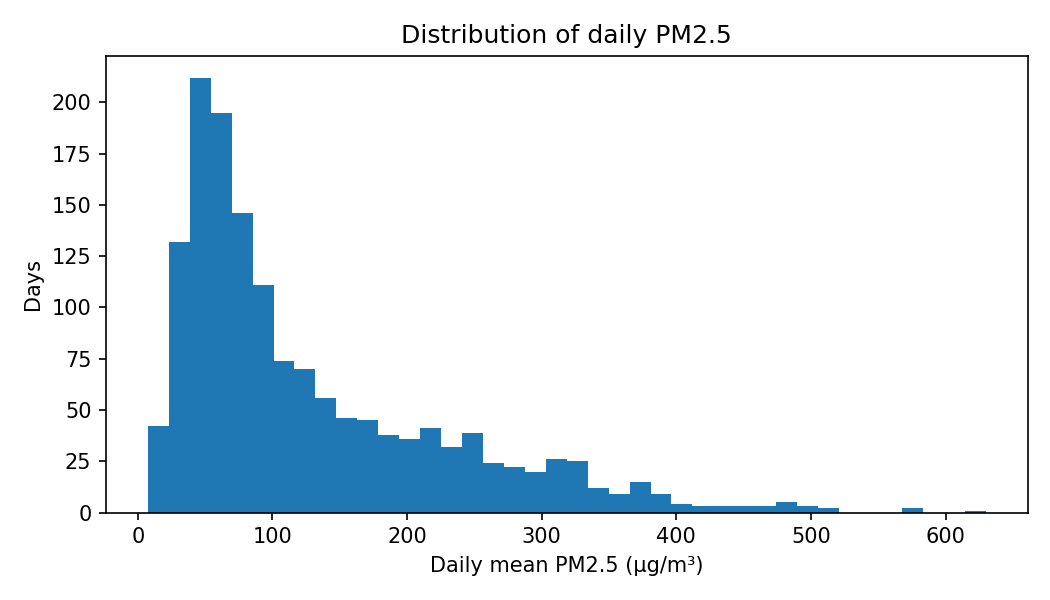
\includegraphics[width=0.78\textwidth]{pm25_distribution.png}
\caption{Distribution of daily mean PM$_{2.5}$ for usable days, Lahore 2019--2025.}
\label{fig:dist}
\end{figure}

\begin{figure}[htbp]
\centering
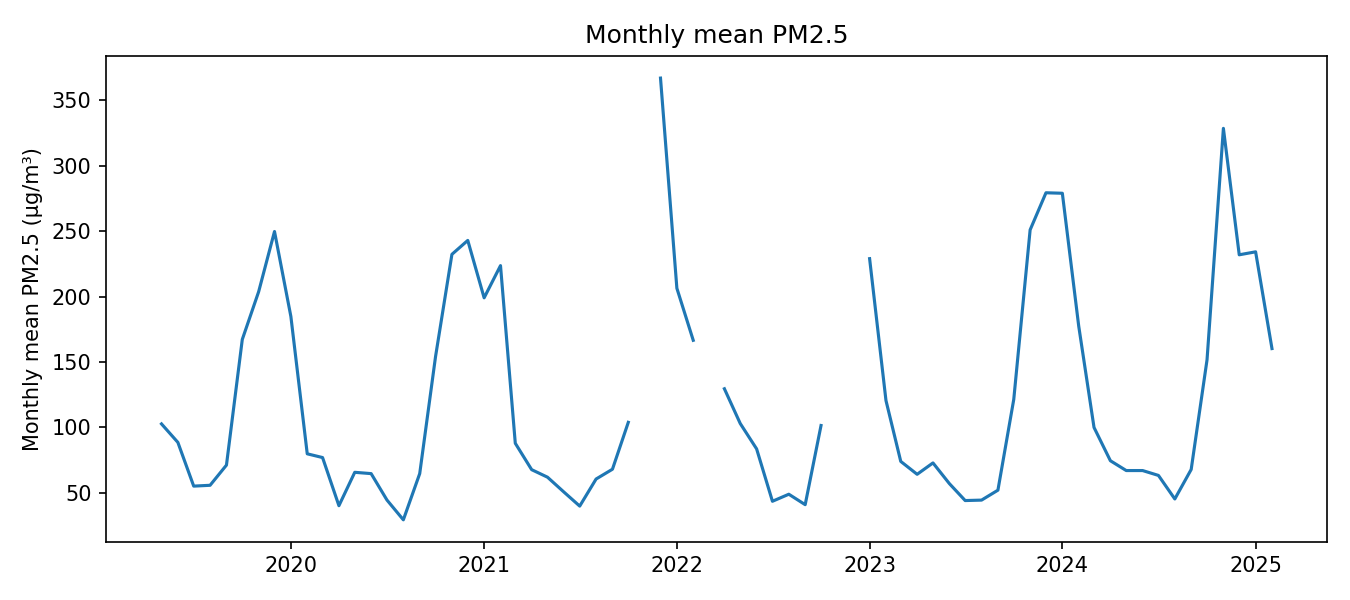
\includegraphics[width=0.86\textwidth]{pm25_monthly.png}
\caption{Monthly mean PM$_{2.5}$. The winter peaks dominate the series; gaps are months with too few usable days.}
\label{fig:monthly}
\end{figure}

\paragraph{Data coverage.}
Coverage is uneven. Figure~\ref{fig:coverage} shows the percentage of usable days in each month: some months are complete, while parts of 2022 and 2023 have very few usable days. This matters for evaluation, because a model trained mostly on winter smog will see a different mix of conditions in a sparse summer month. The time-based split and the per-season error analysis in Phase~3 are designed with this in mind.

\begin{figure}[htbp]
\centering
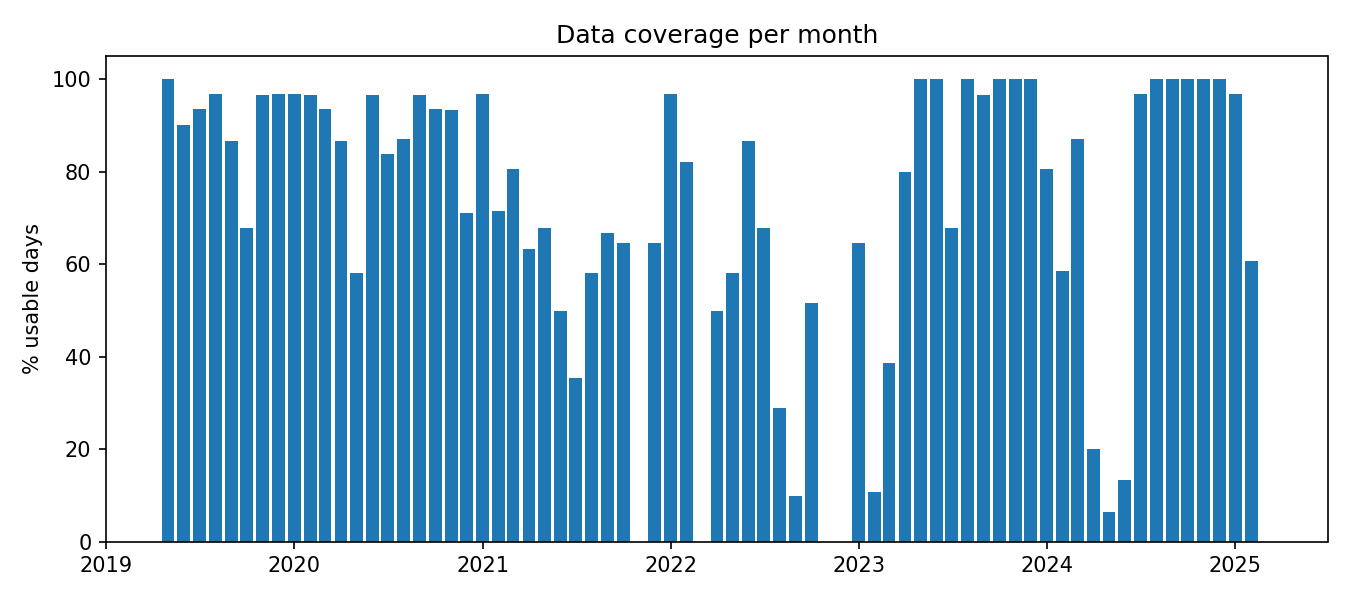
\includegraphics[width=0.86\textwidth]{coverage_by_month.png}
\caption{Percentage of usable days per month. Gaps are months with insufficient valid hourly readings.}
\label{fig:coverage}
\end{figure}

\paragraph{AQI categories.}
Figure~\ref{fig:aqi} and Table~\ref{tab:aqi} show the AQI class distribution. ``Unhealthy'' is the most common class (647 days, 43.0\%), and 1{,}102 days (73.2\%) are ``Unhealthy'' or worse. Only 9 days (0.6\%) are ``Good''. The classes are therefore strongly imbalanced, so overall accuracy would be misleading; Phase~3 will report macro-averaged F1 and per-class recall alongside accuracy.

\begin{figure}[htbp]
\centering
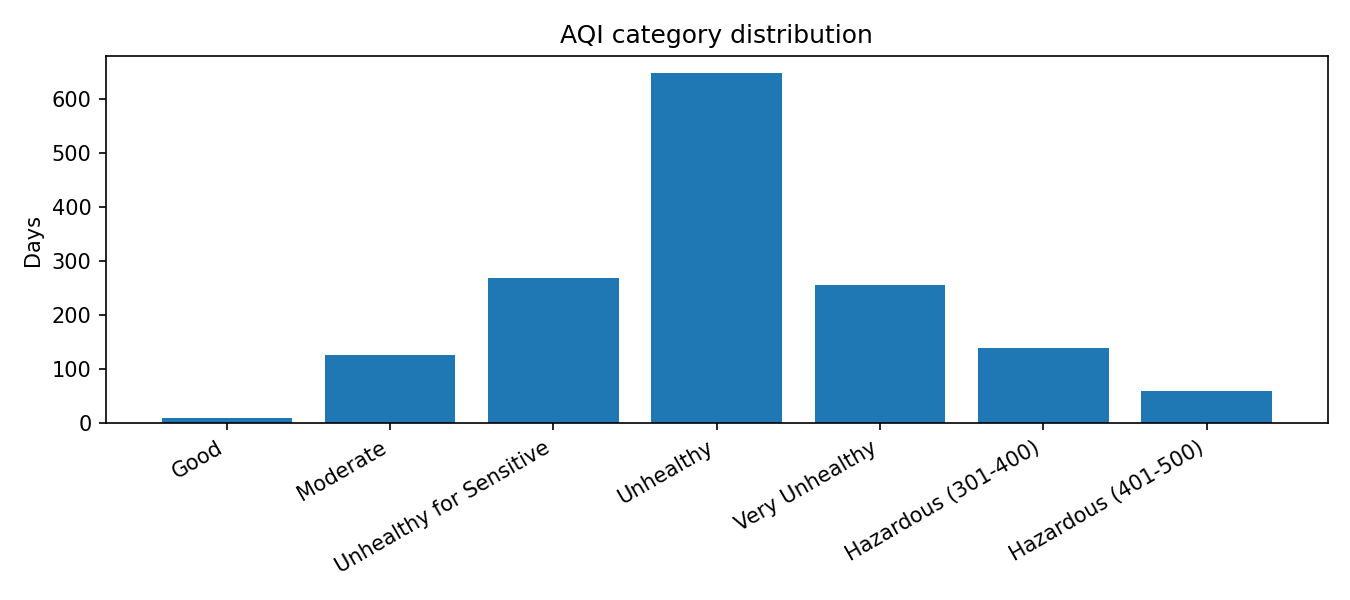
\includegraphics[width=0.86\textwidth]{aqi_class_distribution.png}
\caption{Daily AQI category counts for usable days.}
\label{fig:aqi}
\end{figure}

\begin{table}[htbp]
\centering
\small
\begin{tabular}{L{5.2cm}rr}
\toprule
\textbf{AQI category} & \textbf{Days} & \textbf{Share} \\
\midrule
Good & 9 & 0.6\% \\
Moderate & 126 & 8.4\% \\
Unhealthy for Sensitive Groups & 269 & 17.9\% \\
Unhealthy & 647 & 43.0\% \\
Very Unhealthy & 256 & 17.0\% \\
Hazardous (301--400) & 139 & 9.2\% \\
Hazardous (401--500) & 60 & 4.0\% \\
\midrule
Total & 1{,}506 & 100\% \\
\bottomrule
\end{tabular}
\caption{AQI category distribution for the 1{,}506 usable days.}
\label{tab:aqi}
\end{table}

\paragraph{Relationships with weather.}
Figure~\ref{fig:corr} reports Pearson correlations between daily PM$_{2.5}$ and the meteorological variables. The strongest associations are negative with temperature ($r=-0.64$) and shortwave radiation ($r=-0.50$), and positive with surface pressure ($r=+0.64$). Wind speed is negatively associated ($r=-0.38$) and humidity positively ($r=+0.30$). Figure~\ref{fig:weather} shows the same relationships as scatter plots with linear fits. These patterns are physically consistent: cold, calm, high-pressure days with weak sunlight and little ventilation allow pollution to accumulate, while wind and rain disperse it.

\begin{figure}[htbp]
\centering
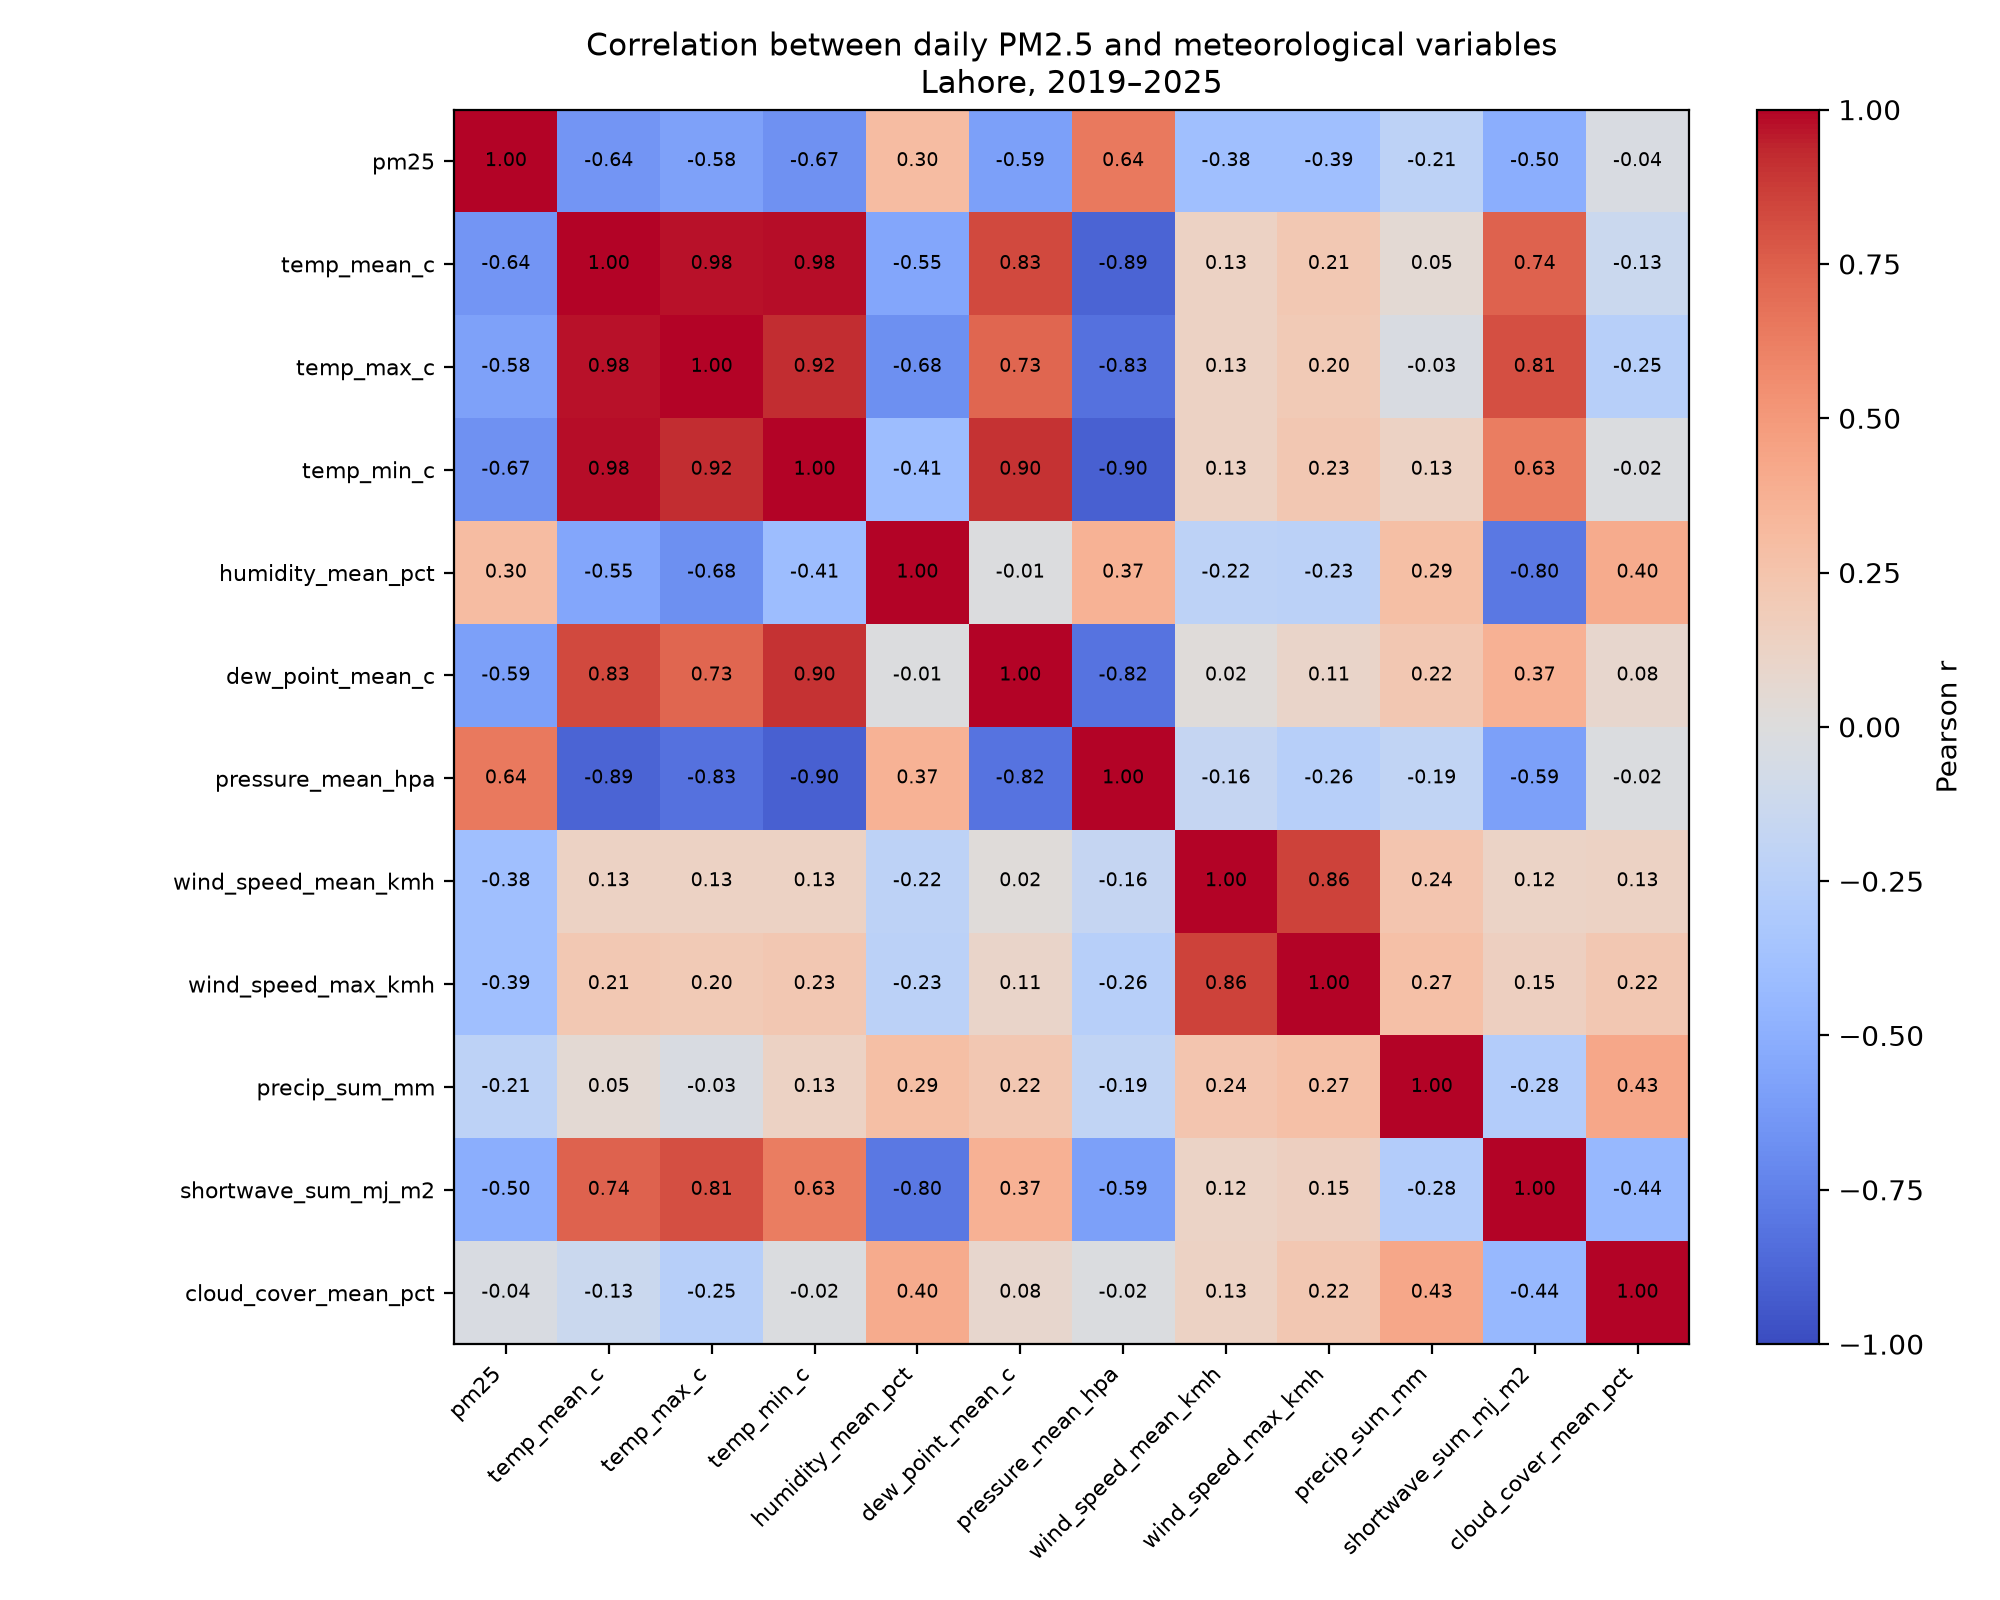
\includegraphics[width=0.86\textwidth]{correlation_heatmap.png}
\caption{Pearson correlation matrix for daily PM$_{2.5}$ and meteorological variables.}
\label{fig:corr}
\end{figure}

\begin{figure}[htbp]
\centering
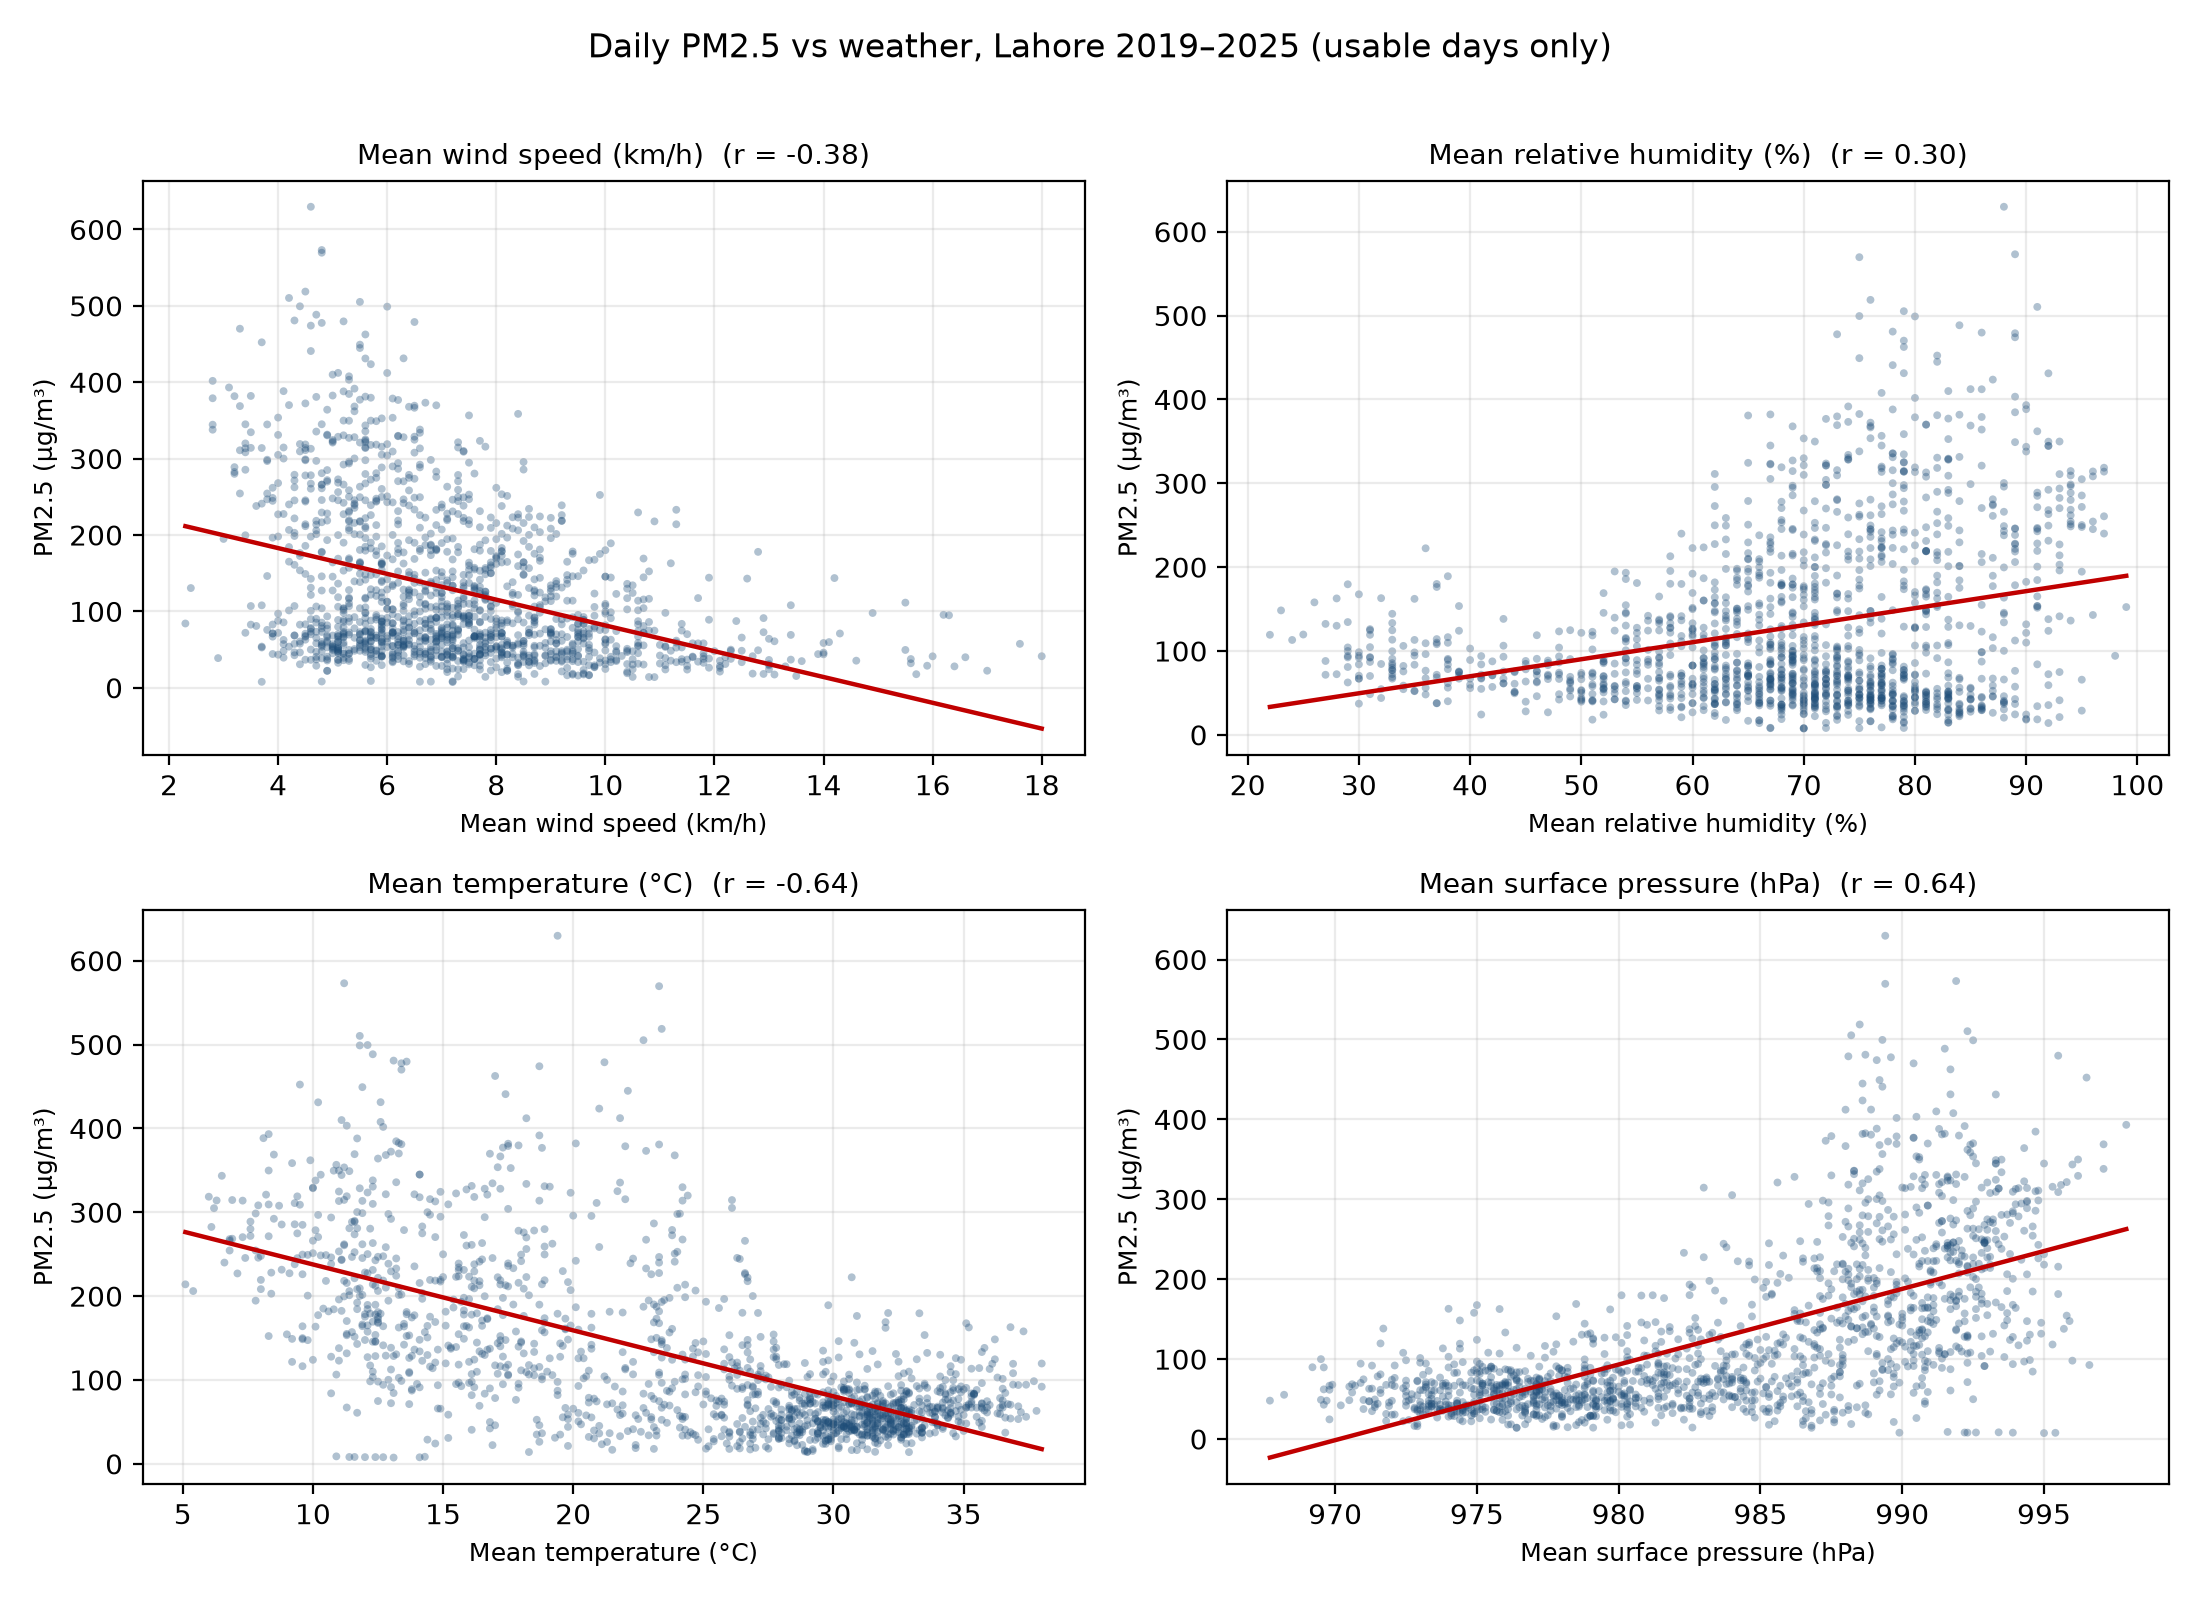
\includegraphics[width=0.92\textwidth]{weather_vs_pm25.png}
\caption{Daily PM$_{2.5}$ against wind speed, humidity, temperature and pressure, with linear fits.}
\label{fig:weather}
\end{figure}

\paragraph{What the EDA implies for modelling.}
Three points follow. First, the seasonal cycle is strong enough that season and calendar features are necessary, not optional. Second, persistence is likely to be the hardest baseline to beat, which is why Phase~1 commits to reporting it. Third, the weather relationships are correlations, not causal effects; the models will be evaluated on held-out years rather than on their ability to fit these patterns.

\subsection{Data Limitations and Ethical Considerations}

\begin{itemize}
  \item \textbf{One monitor, not a city.} The target comes from a single US Diplomatic Post monitor. It is a useful reference series but does not represent every neighbourhood in Lahore.
  \item \textbf{Substantial gaps.} 607 of 2{,}113 calendar days (28.7\%) do not have enough valid hours. Coverage is uneven across months, so evaluation must report results by season as well as overall.
  \item \textbf{Station file gaps.} The station AQI is missing on 221 of 1{,}644 days (13.4\%), including a 47-day gap in the 2021 smog season.
  \item \textbf{Modelled data is not measured data.} The CAMS products are used for comparison only. On the 632 days shared with the monitor, the modelled daily series averaged 0.54 of the monitor's level (median daily ratio 0.61) and under-read smog peaks, so it cannot substitute for observations.
  \item \textbf{Calendar proxies are approximate.} Ramadan and Eid dates follow published calendars but can shift by a day with moon sighting; public holidays are a simplification. Traffic is not observed directly.
  \item \textbf{Licences.} The Zenodo dataset is CC0-1.0 and Open-Meteo/ERA5 is CC BY 4.0. The Kaggle \texttt{aadbutt} dataset states an unknown licence, and the GitHub station repository states no licence. We therefore attribute both sources and keep raw files out of the public repository rather than redistributing them.
  \item \textbf{Not medical advice.} The application provides cautious, category-based guidance and does not replace official health advisories.
\end{itemize}


\begin{thebibliography}{9}

\bibitem{majeed2024lahore}
R. Majeed, M. S. Anjum, M. Imad-ud-din, S. Malik, M. N. Anwar, B. Anwar, and M. F. Khokhar,
``Solving the mysteries of Lahore smog: the fifth season in the country,''
\emph{Frontiers in Sustainable Cities}, vol.~5, art.~1314426, 2024.
doi:10.3389/frsc.2023.1314426.

\bibitem{who2024ambient}
World Health Organization,
``Ambient (outdoor) air pollution,'' fact sheet, 24 October 2024.
[Online]. Available: \url{https://www.who.int/news-room/fact-sheets/detail/ambient-(outdoor)-air-quality-and-health}

\bibitem{epa_pm_basics}
U.S. Environmental Protection Agency,
``Particulate Matter (PM) Basics.''
[Online]. Available: \url{https://www.epa.gov/pm-pollution/particulate-matter-pm-basics}

\bibitem{epa_aqi_tad}
U.S. Environmental Protection Agency,
``Technical Assistance Document for the Reporting of Daily Air Quality -- the Air Quality Index (AQI),'' EPA-454/B-18-007, September 2018.
[Online]. Available: \url{https://www.airnow.gov/sites/default/files/2020-05/aqi-technical-assistance-document-sept2018.pdf}

\bibitem{waqas2024lahore}
H. M. S. Waqas, T. Naz, K. Shahid, A. Yaqoob, and M. B. Ahmad,
``Time series forecasting of air quality index in Lahore: a machine learning perspective with Facebook Prophet model,''
\emph{International Journal of Scientific Research in Science and Technology}, vol.~11, no.~5, pp.~219--226, 2024.
doi:10.32628/IJSRST2411598.

\end{thebibliography}

\end{document}
